\section{Thermal Diffusivity Sensitivity Study}\label{sec:diffusivity}
The thermal diffusivity, $\alpha_{th}$ of geologic repository host media 
describes the tendency of thermal energy to diffuse through, and therefore be 
deposited, in the medium.

In the creation of the \gls{STC} database, the thermal diffusivity was varied 
across a broad domain for each isotope, $i$, package spacing, $s$, limiting 
radius $r_{calc}$, and thermal conductivity $K_{th}$, considered.  By 
varying the thermal diffusivity of the repository model from $0.1-3\times 
10^{-6} [m^2\cdot s^{-1}]$, this sensitivity analysis succeeds in capturing the domain of 
thermal diffusivities witnessed in high thermal diffusivity salt deposits as 
well as low thermal diffusivity clays.

\begin{figure}[htbp!]
\begin{center}
%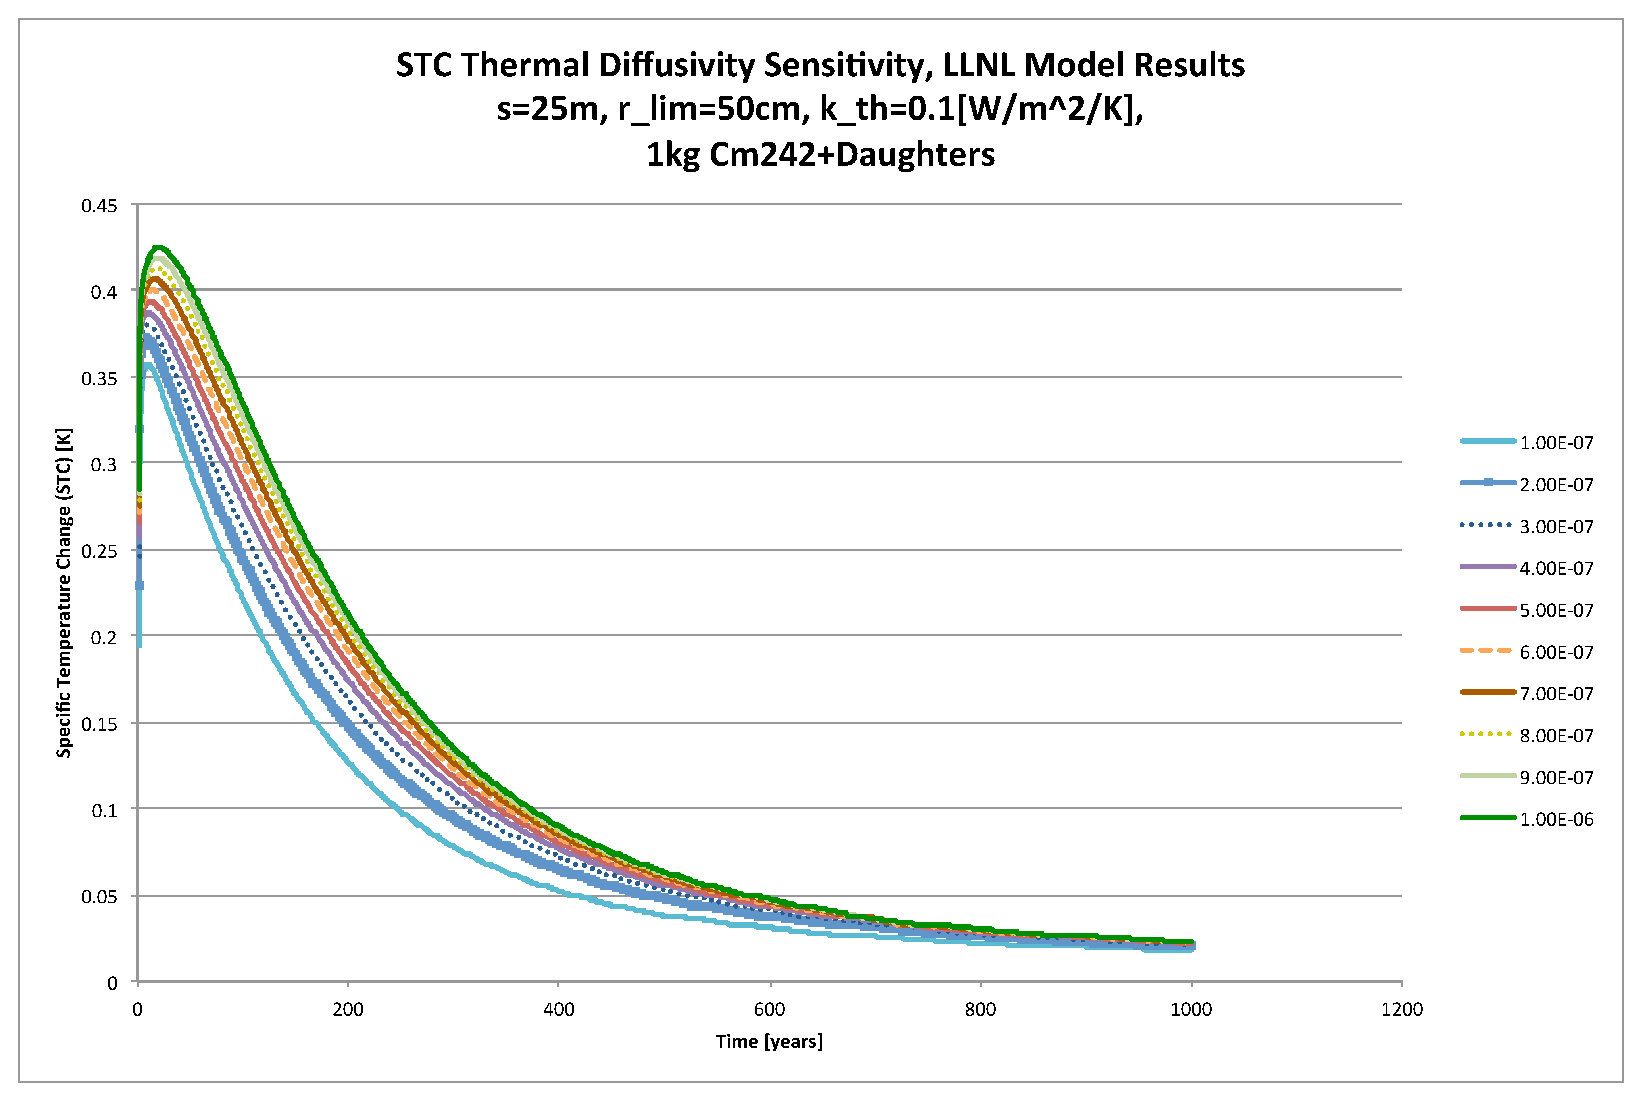
\includegraphics[width=0.7\textwidth]{./chapters/demonstration/diffusivity/Cm242alpha_kth_low.eps}
\end{center}
\caption[$K_{th}$ Sensitivity for Low $\alpha_{th}$]{Increased thermal diffusivity decreases thermal energy deposition 
(here represented by \gls{STC}) in the near field (here $r_{calc} = 0.5m$).}
\label{fig:Cm242alpha_kth_low}
\end{figure}


Figure \ref{fig:Cm242alpha_kth_low} shows the trend, visible for all isotopes, 
that increased thermal diffusivity of a medium decreases thermal energy 
deposition in the near field. This indicates, then that thermal diffusivity is 
an important parameter for repository geolgic medium selection. The effect is 
accentuated by high thermal conductivities, as seen in 
Figure \ref{fig:Cm242alpha_kth_high}

\begin{figure}[htbp!]
\begin{center}
%\includegraphics[width=0.7\textwidth]{./chapters/demonstration/diffusivity/Cm242alpha_kth_high.eps}
\end{center}
\caption[$K_{th}$ Sensitivity for High $\alpha_{th}$]{Increased thermal diffusivity decreases thermal energy deposition 
(here represented by \gls{STC}) in the near field (here $r_{calc} = 0.5m$).}
\label{fig:Cm242alpha_kth_high}
\end{figure}


